\section{Descripción del contexto histórico y actual del Paraguay}

\subsection{Contexto Demográfico}\subsubsection{Población}

El Censo Nacional de Población y Viviendas en la República del Paraguay
se realiza cada 10 años, siendo el Instituto Nacional de Estadística
(INE) la institución encargada de llevarlo a cabo.

Se utilizan como insumos para este estudio, tanto el censo del año 2002
como el último censo realizado en nuestro país en el año 2012 con sus
proyecciones (periodo 2000-2025) de la población nacional por sexo y
edad, según áreas urbana y rural; así como la Encuesta Permanente de
Hogares (EPH) de los años 2013 al 2020.

Según estas proyecciones, la población total del Paraguay al año 2020 se
estima en 7,25 millones, de los cuales 3,65 millones son hombres y 3,60
millones son mujeres. Respecto a la distribución por área de residencia,
4,53 millones son del área urbana y 2,72 millones del área rural.

\begin{table}[H]
\begin{center}
\footnotesize
\caption{\bf{Población total por año, según sexo. Periodo 2000-2025}}
\begin{tabular}{l|rrrrrr}
\begin{tabular}{llll}
\cline{1-4}
\multicolumn{1}{c}{} &
  \multicolumn{3}{|c}{Sexo} \\
\multicolumn{1}{c}{} &
  \multicolumn{1}{|r}{Hombres} &
  \multicolumn{1}{r}{Mujeres} &
  \multicolumn{1}{r}{Total} \\
\cline{1-4}
\multicolumn{1}{l}{Año} &
  \multicolumn{1}{|r}{} &
  \multicolumn{1}{r}{} &
  \multicolumn{1}{r}{} \\
\multicolumn{1}{l}{\hspace{1em}2000} &
  \multicolumn{1}{|r}{2.671.656} &
  \multicolumn{1}{r}{2.612.824} &
  \multicolumn{1}{r}{5.284.480} \\
\multicolumn{1}{l}{\hspace{1em}2001} &
  \multicolumn{1}{|r}{2.722.569} &
  \multicolumn{1}{r}{2.662.432} &
  \multicolumn{1}{r}{5.385.002} \\
\multicolumn{1}{l}{\hspace{1em}2002} &
  \multicolumn{1}{|r}{2.772.953} &
  \multicolumn{1}{r}{2.711.657} &
  \multicolumn{1}{r}{5.484.610} \\
\multicolumn{1}{l}{\hspace{1em}2003} &
  \multicolumn{1}{|r}{2.822.895} &
  \multicolumn{1}{r}{2.760.589} &
  \multicolumn{1}{r}{5.583.484} \\
\multicolumn{1}{l}{\hspace{1em}2004} &
  \multicolumn{1}{|r}{2.872.516} &
  \multicolumn{1}{r}{2.809.356} &
  \multicolumn{1}{r}{5.681.872} \\
\multicolumn{1}{l}{\hspace{1em}2005} &
  \multicolumn{1}{|r}{2.921.813} &
  \multicolumn{1}{r}{2.857.956} &
  \multicolumn{1}{r}{5.779.769} \\
\multicolumn{1}{l}{\hspace{1em}2006} &
  \multicolumn{1}{|r}{2.970.854} &
  \multicolumn{1}{r}{2.906.469} &
  \multicolumn{1}{r}{5.877.323} \\
\multicolumn{1}{l}{\hspace{1em}2007} &
  \multicolumn{1}{|r}{3.019.704} &
  \multicolumn{1}{r}{2.954.962} &
  \multicolumn{1}{r}{5.974.666} \\
\multicolumn{1}{l}{\hspace{1em}2008} &
  \multicolumn{1}{|r}{3.068.356} &
  \multicolumn{1}{r}{3.003.425} &
  \multicolumn{1}{r}{6.071.781} \\
\multicolumn{1}{l}{\hspace{1em}2009} &
  \multicolumn{1}{|r}{3.116.847} &
  \multicolumn{1}{r}{3.051.910} &
  \multicolumn{1}{r}{6.168.757} \\
\multicolumn{1}{l}{\hspace{1em}2010} &
  \multicolumn{1}{|r}{3.165.316} &
  \multicolumn{1}{r}{3.100.561} &
  \multicolumn{1}{r}{6.265.877} \\
\multicolumn{1}{l}{\hspace{1em}2011} &
  \multicolumn{1}{|r}{3.213.839} &
  \multicolumn{1}{r}{3.149.438} &
  \multicolumn{1}{r}{6.363.276} \\
\multicolumn{1}{l}{\hspace{1em}2012} &
  \multicolumn{1}{|r}{3.262.466} &
  \multicolumn{1}{r}{3.198.575} &
  \multicolumn{1}{r}{6.461.041} \\
\multicolumn{1}{l}{\hspace{1em}2013} &
  \multicolumn{1}{|r}{3.311.123} &
  \multicolumn{1}{r}{3.247.904} &
  \multicolumn{1}{r}{6.559.027} \\
\multicolumn{1}{l}{\hspace{1em}2014} &
  \multicolumn{1}{|r}{3.359.806} &
  \multicolumn{1}{r}{3.297.426} &
  \multicolumn{1}{r}{6.657.232} \\
\multicolumn{1}{l}{\hspace{1em}2015} &
  \multicolumn{1}{|r}{3.408.566} &
  \multicolumn{1}{r}{3.347.190} &
  \multicolumn{1}{r}{6.755.756} \\
\multicolumn{1}{l}{\hspace{1em}2016} &
  \multicolumn{1}{|r}{3.457.365} &
  \multicolumn{1}{r}{3.397.170} &
  \multicolumn{1}{r}{6.854.536} \\
\multicolumn{1}{l}{\hspace{1em}2017} &
  \multicolumn{1}{|r}{3.506.242} &
  \multicolumn{1}{r}{3.447.404} &
  \multicolumn{1}{r}{6.953.646} \\
\multicolumn{1}{l}{\hspace{1em}2018} &
  \multicolumn{1}{|r}{3.555.140} &
  \multicolumn{1}{r}{3.497.843} &
  \multicolumn{1}{r}{7.052.983} \\
\multicolumn{1}{l}{\hspace{1em}2019} &
  \multicolumn{1}{|r}{3.604.135} &
  \multicolumn{1}{r}{3.548.568} &
  \multicolumn{1}{r}{7.152.703} \\
\multicolumn{1}{l}{\hspace{1em}2020} &
  \multicolumn{1}{|r}{3.653.156} &
  \multicolumn{1}{r}{3.599.516} &
  \multicolumn{1}{r}{7.252.672} \\
\multicolumn{1}{l}{\hspace{1em}2021} &
  \multicolumn{1}{|r}{3.702.281} &
  \multicolumn{1}{r}{3.650.758} &
  \multicolumn{1}{r}{7.353.038} \\
\multicolumn{1}{l}{\hspace{1em}2022} &
  \multicolumn{1}{|r}{3.751.447} &
  \multicolumn{1}{r}{3.702.248} &
  \multicolumn{1}{r}{7.453.695} \\
\multicolumn{1}{l}{\hspace{1em}2023} &
  \multicolumn{1}{|r}{3.800.735} &
  \multicolumn{1}{r}{3.754.061} &
  \multicolumn{1}{r}{7.554.796} \\
\multicolumn{1}{l}{\hspace{1em}2024} &
  \multicolumn{1}{|r}{3.850.075} &
  \multicolumn{1}{r}{3.806.140} &
  \multicolumn{1}{r}{7.656.215} \\
\multicolumn{1}{l}{\hspace{1em}2025} &
  \multicolumn{1}{|r}{3.899.638} &
  \multicolumn{1}{r}{3.858.624} &
  \multicolumn{1}{r}{7.758.263} \\
\cline{1-4}
\end{tabular}

\end{tabular}
                    \item \footnotesize Fuente : Instituto Nacional de Estadística.
\end{center}
\end{table}

\begin{figure}[H]
\begin{center}
                    \caption{Población total por año, según sexo. Periodo 2000-2025}
                    \includegraphics[scale=0.45]{indicadoresINE_pob_sexo_serie.png}
                                    \item \footnotesize Fuente : Instituto Nacional de Estadística.
                    \end{center}
\end{figure}

En la pirámide poblacional del año 2020 realizada con los datos de las
proyecciones de población, se puede apreciar una base ancha y cúspide
angosta, lo que representa una población mayoritariamente joven con un
55,85\% de personas menores de 30 años.

\textbf{agregar los gráficos de proyección de nacimientos y fallecimientos, el de evolución demográfica y el de proyección de participación según grupos de edad}

\begin{figure}[H]
\begin{center}
                    \caption{Pirámide poblacional. Año 2020}
                    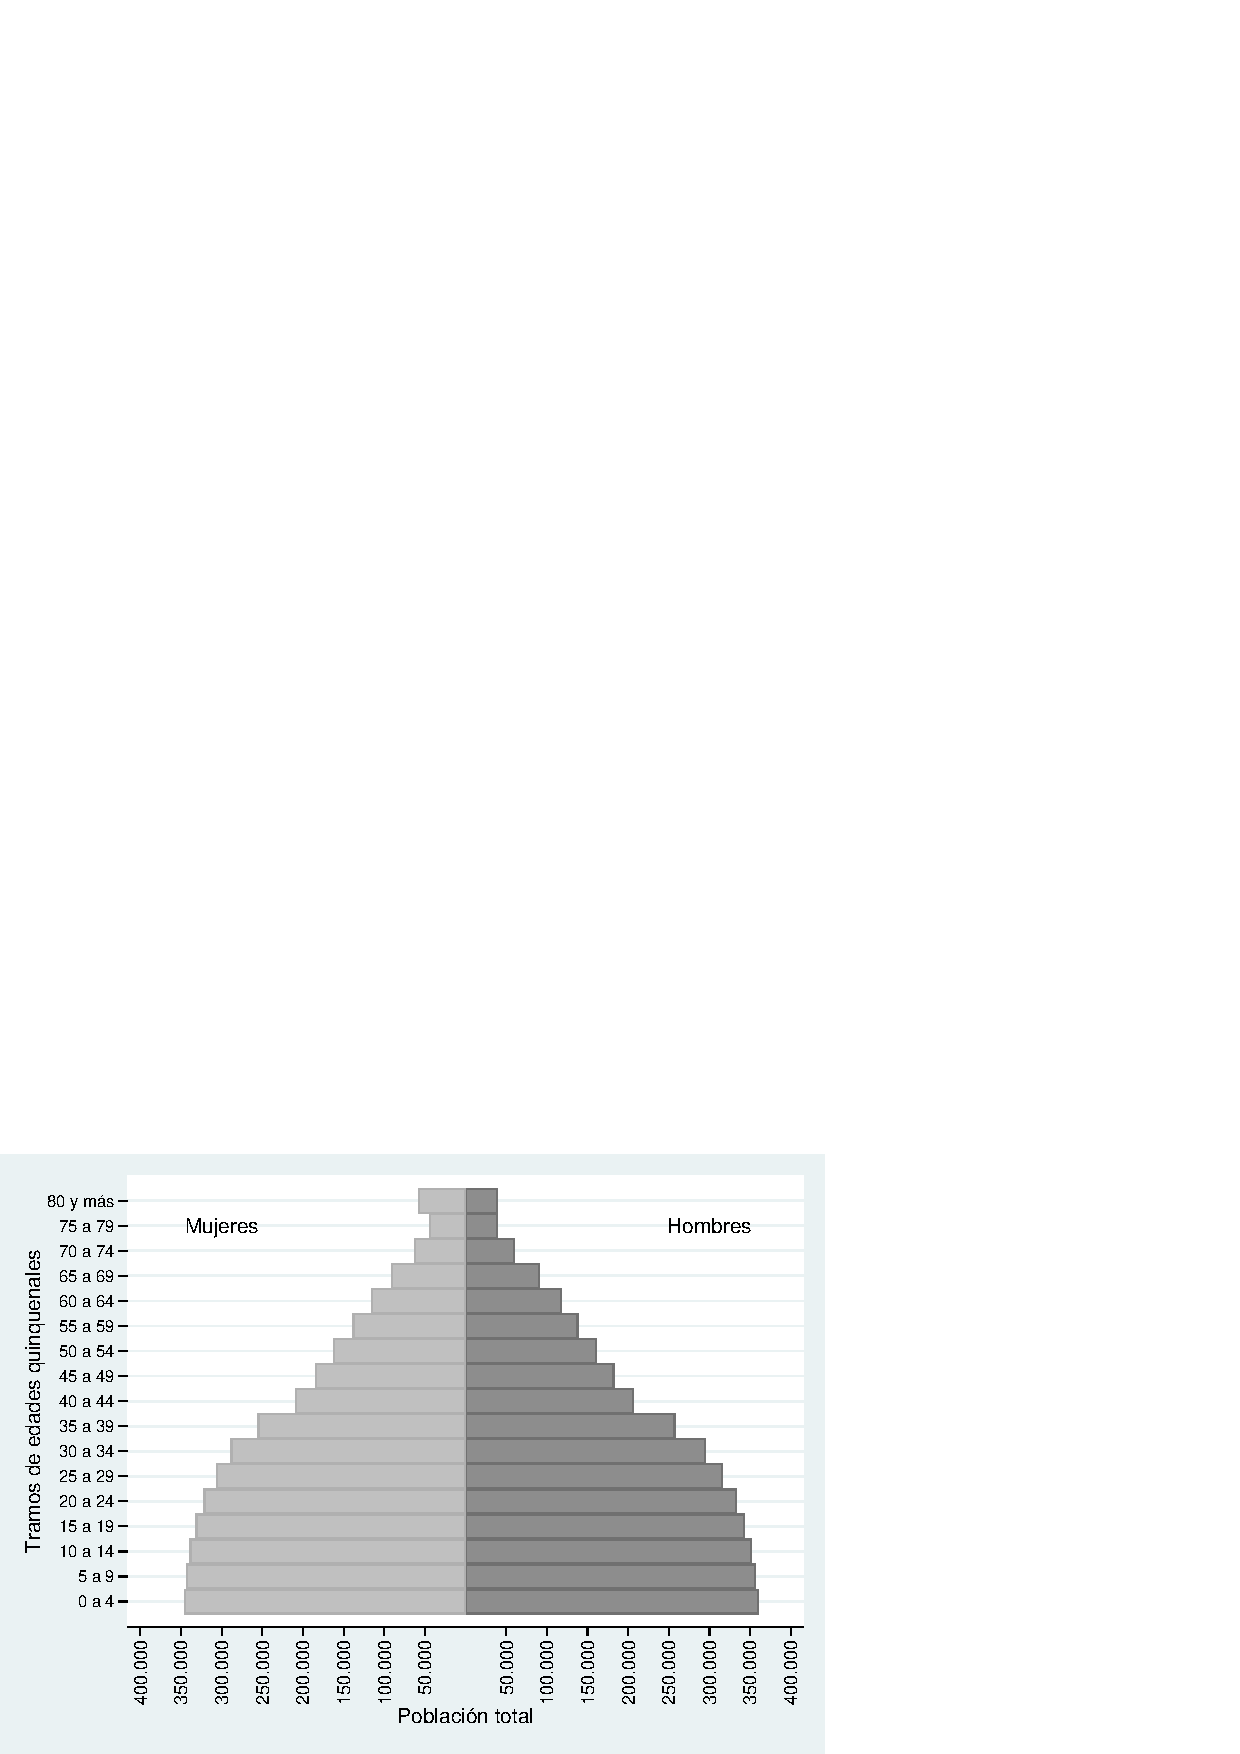
\includegraphics[scale=0.45]{indicadoresINE_pobtot_piramide.png}
                                    \item \footnotesize Fuente : Instituto Nacional de Estadística.
                    \end{center}
\end{figure}

\subsubsection{Esperanza de vida - Mortalidad}

La Esperanza de Vida es el promedio de años que se espera viva una
persona a partir de la edad que tiene, por lo que a la hora de analizar
un Sistema de Jubilaciones y Pensiones se necesita no sólo saber la
esperanza de vida al nacer sino también la esp eranza de vida de la
persona al momento de jubilarse, ya que esto representa cuantos años en
promedio se estarán pagando las jubilaciones.

En la evolución de la Esperanza de Vida al nacer por sexo, se puede
apreciar dos puntos relevantes: primero, en ambos sexos existe un
incremento en la esperanza de vida al nacer; y segundo, las mujeres
siempre tienen una expectativa de vida superior a l a de los hombres a
lo largo del periodo considerado.

Una expectativa de vida superior en las mujeres es una situación similar
a la que se presenta en los países de la región y en los países
desarrollados. El incremento de los años que se espera vivir en promedio
en Paraguay también es una evolución natur al debido a una mejora
continua en la calidad de vida mediante el acceso a los servicios
sanitarios (inmunizaciones, asistencia pediátrica) y servicios públicos
de suministro (agua, electricidad, alcantarillado sanitario).

La esperanza de vida al nacer de un hombre en Paraguay en el 2001 era de
67,6 años, mientras que la de una mujer era de 72,8 años. Para el año
2020 se estima que la esperanza de vida del hombre aumentó en 4,1 años
llegando a 71,7; en tanto que para la m ujer se incrementó en 4,9 años,
alcanzando la edad de 77,7. Esto evidencia una diferencia promedio en la
esperanza de vida de 5,6 años a favor de las mujeres a lo largo del
periodo analizado.

\begin{figure}[H]
\begin{center}
                    \caption{Esperanza de vida al nacer. Periodo 2001-2025}
                    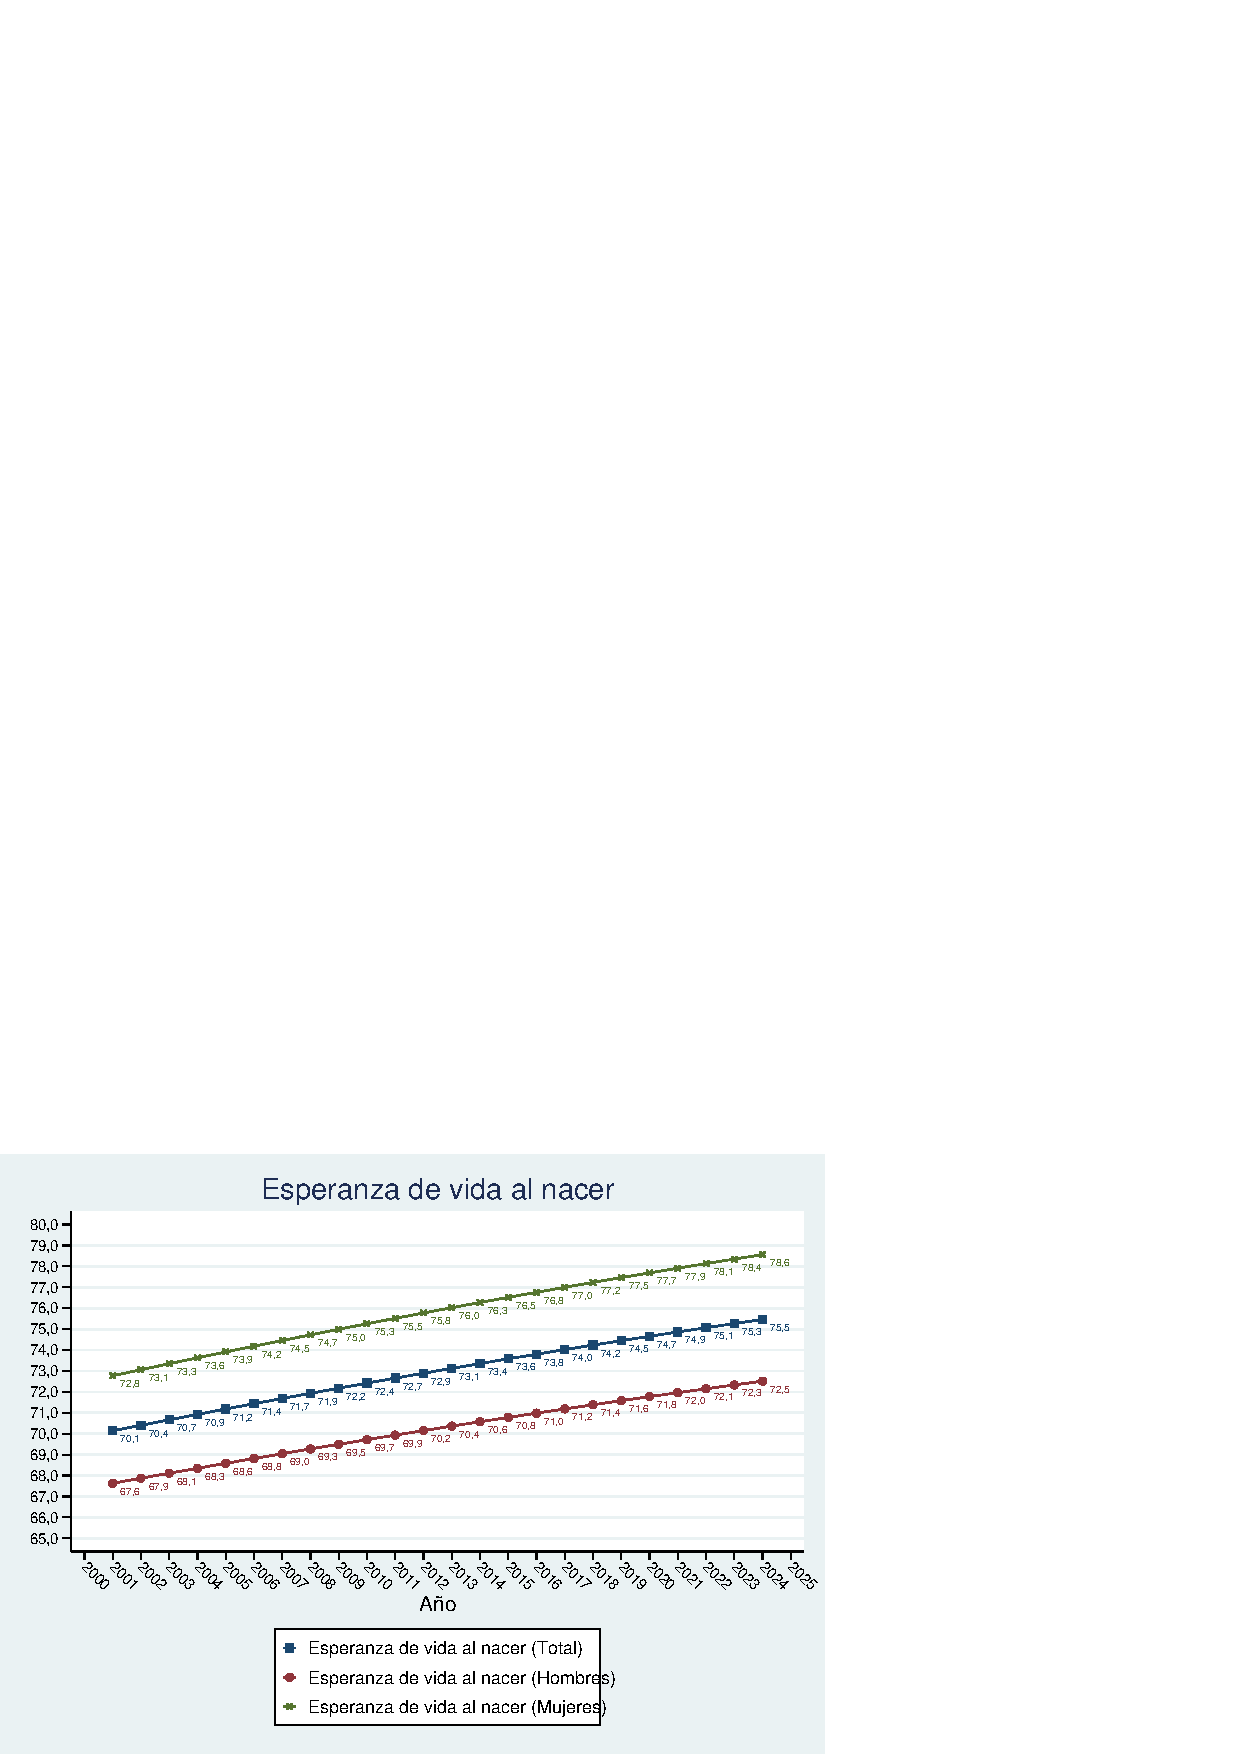
\includegraphics[scale=0.45]{INE_indic_ev0.png}
                                    \item \footnotesize Fuente : Instituto Nacional de Estadística.
                    \end{center}
\end{figure}

El número de muertes para el año 2001 en el Paraguay ascendía a 33.185.
Para el año 2025 se estima un incremento de 32,1\% en dicha cifra,
alcanzado un valor aproximado de 43.836 muertes por año.

\begin{figure}[H]
\begin{center}
                    \caption{Número de muertes por año. Periodo 2001-2025}
                    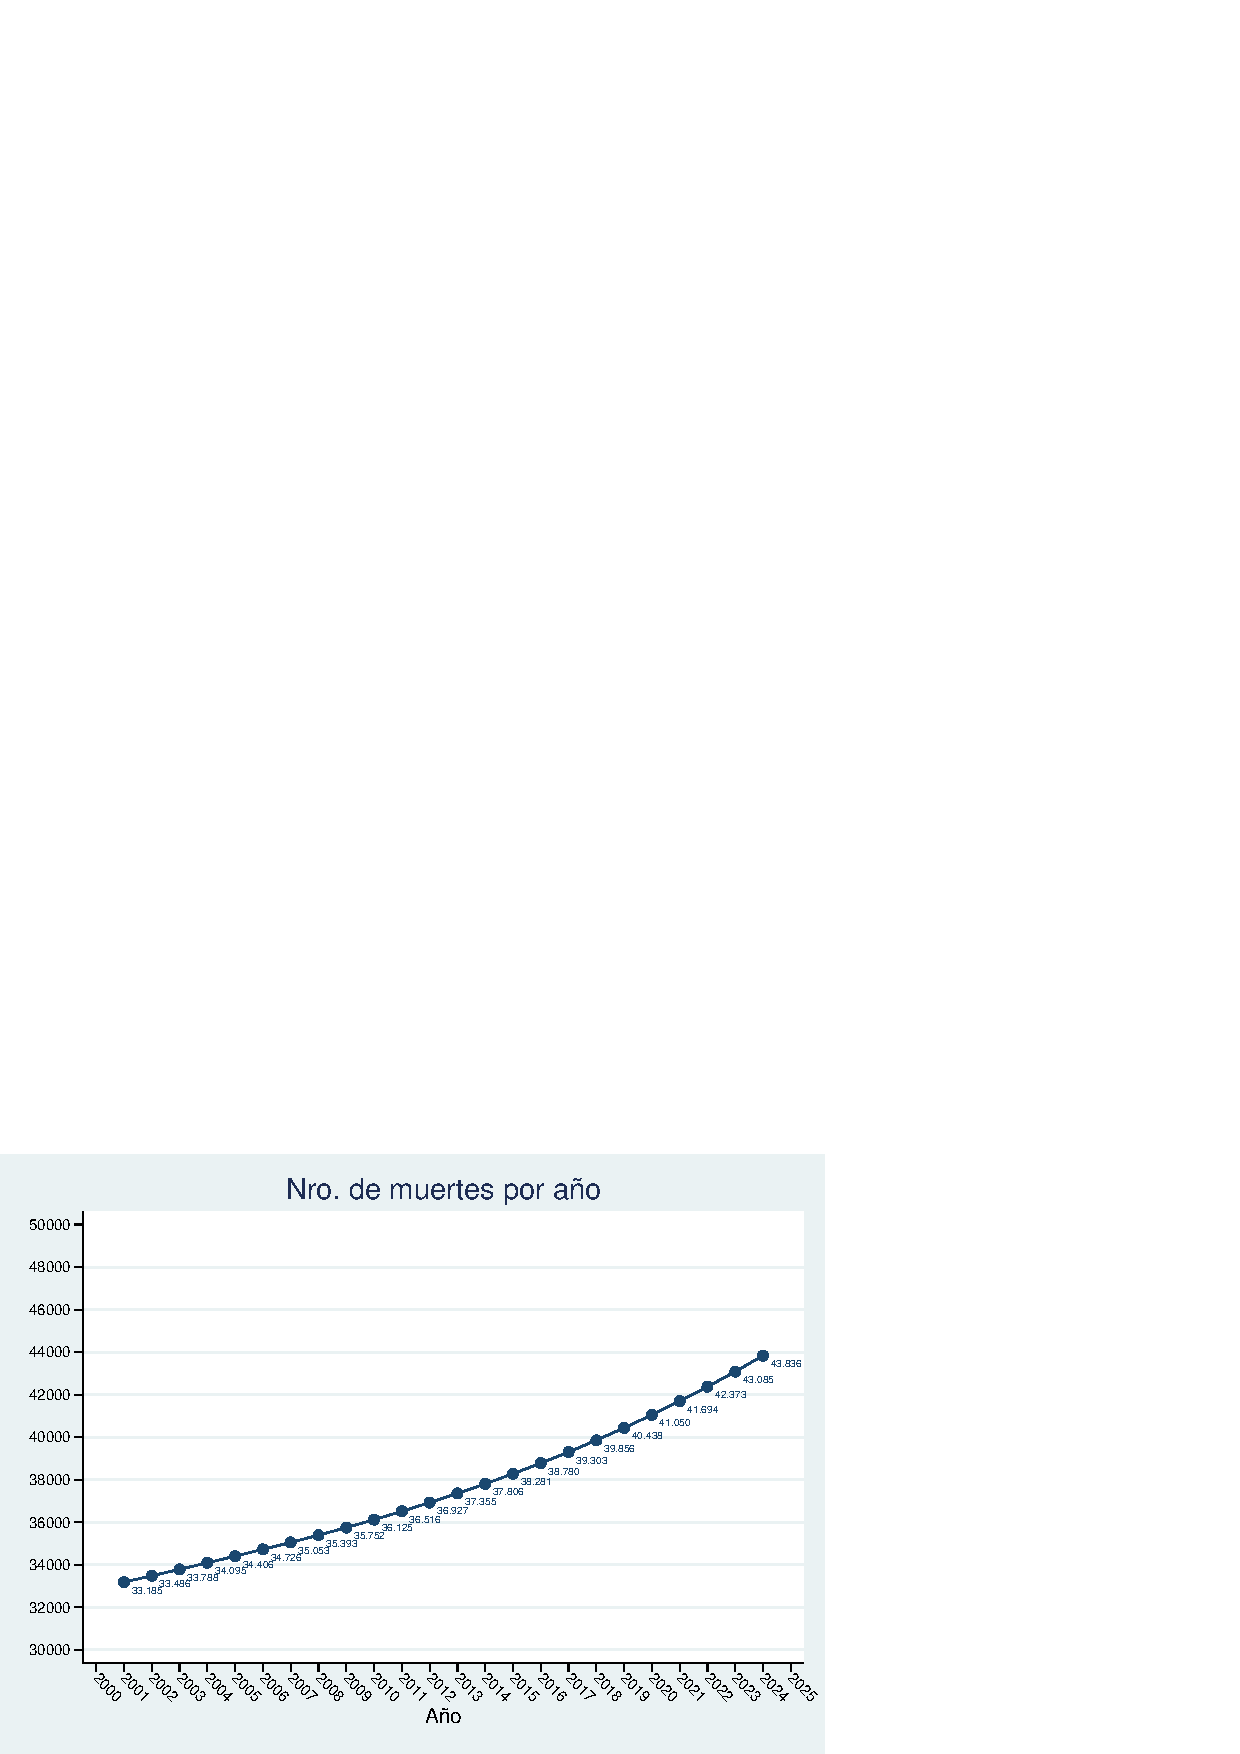
\includegraphics[scale=0.45]{INE_indic_nromuertesanual.png}
                                    \item \footnotesize Fuente : Instituto Nacional de Estadística.
                    \end{center}
\end{figure}

Si bien existe una mejora en la probabilidad de supervivencia para todas
las edades, la principal mejora se da en las edades más jóvenes, lo que
da indicio de que la pirámide poblacional irá ensanchándose, es decir,
la forma de la distribución irá cambi ando lentamente de una forma
piramidal hacia una más rectangular.

En cuanto a la evolución de la esperanza de vida a los 60 años para
hombres y mujeres en el Paraguay, en el año 2000 se pagaba jubilaciones
a una persona de 60 años, en promedio durante 19,4 años si era hombre y
21,9 si era mujer, mientras que para el a ño 2020 se adiciona 1,4 años
para los hombres y 2,3 años a las mujeres para el mismo fin.

\begin{figure}[H]
\begin{center}
                    \caption{Esperanza de vida a los 60 años por sexo, según periodo}
                    \includegraphics[scale=0.45]{INE_indic_ex_periodo_60.png}
                    \item \footnotesize Fuente : Instituto Nacional de Estadística.
                    \end{center}
\end{figure}

\subsubsection{Fecundidad}

De manera sencilla, se puede definir la Tasa Global de Fecundidad
(TGF)\footnote{ De manera formal, CELADE define la Tasa Global de Fecundidad como "el número de hijos que en promedio tendría una mujer de una cohorte hipotética de mujeres que durante su
 vida fértil tuvieran sus hijos de acuerdo a las tasas de fecundidad por edad del período en estudio y no estuvieran expuestas a riesgos de mortalidad desde el nacimiento hasta el término del período fértil" (CELADE, 2017).}
como ``el número de hijos en promedio que tiene una mujer durante toda
su vida
fértil\footnote{ Se considera que la mujer se encuentra en edad reproductiva (edad fértil) entre los 15 y 49 años.}''.

Si bien a la hora de proyectar la población se utilizan tasas de
fecundidad por edad simple, la TGF es un indicador de la tendencia en la
fecundidad y finalmente cómo se espera que evolucione la población.

Al presentar la evolución de la TGF en Paraguay, se puede apreciar una
clara tendencia decreciente, pasando de 3,4 hijos por mujer en el año
2001 a 2,4 hijos por mujer en el año 2020.

El aumento de la esperanza de vida va acompañado de una disminución de
la tasa de fecundidad, factor que también incide en el ensanchamiento de
la pirámide de población.

Según datos del INE, para el año 2025 se estima un total de 145.228
nacimientos en el país.

\begin{figure}[H]
\begin{center}
                    \caption{Número de nacimientos por año. Periodo 2001-2025}
                    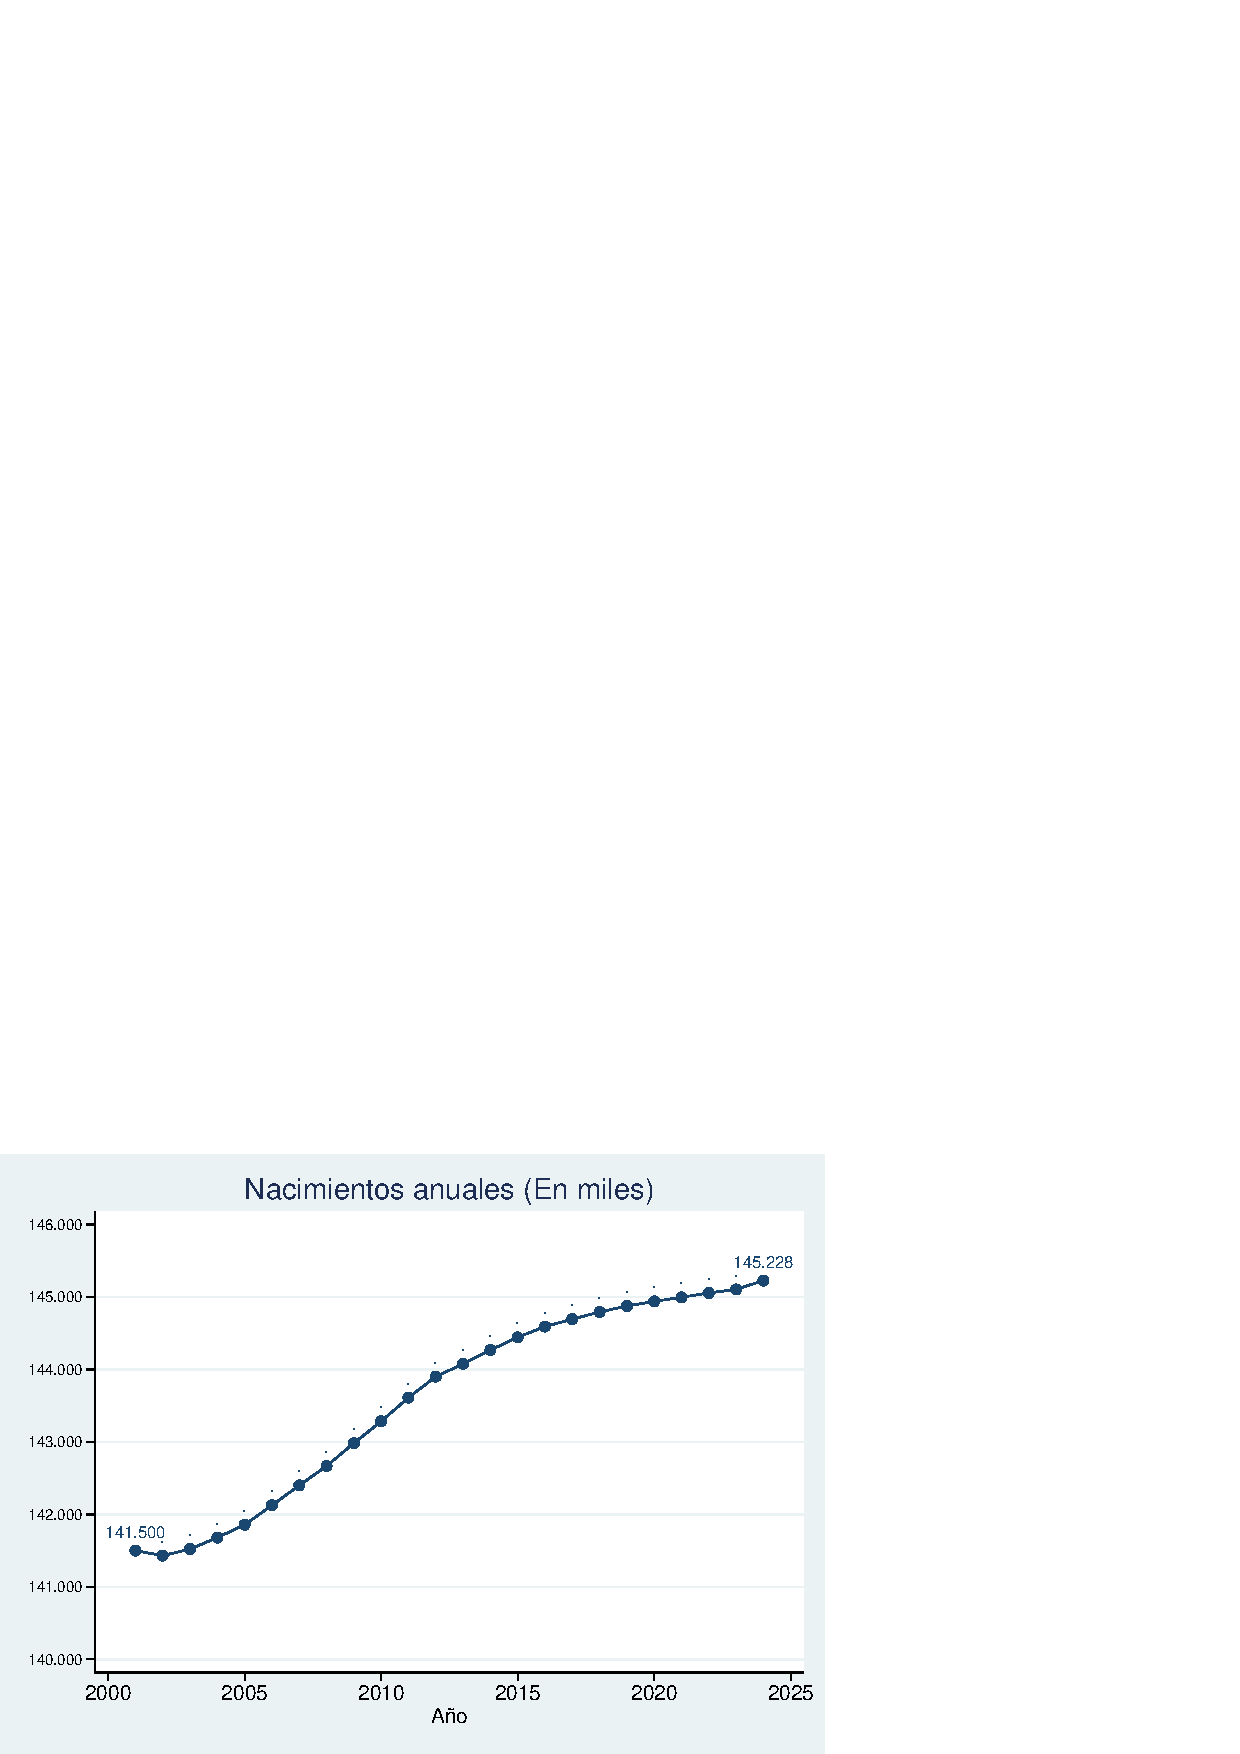
\includegraphics[scale=0.45]{INEnronacanual.png}
                                    \item \footnotesize Fuente : Instituto Nacional de Estadísticas.

                    \end{center}
\end{figure}

\begin{figure}[H]
\begin{center}
                    \caption{Tasa global de fecundidad. Periodo 2001-2025}
                    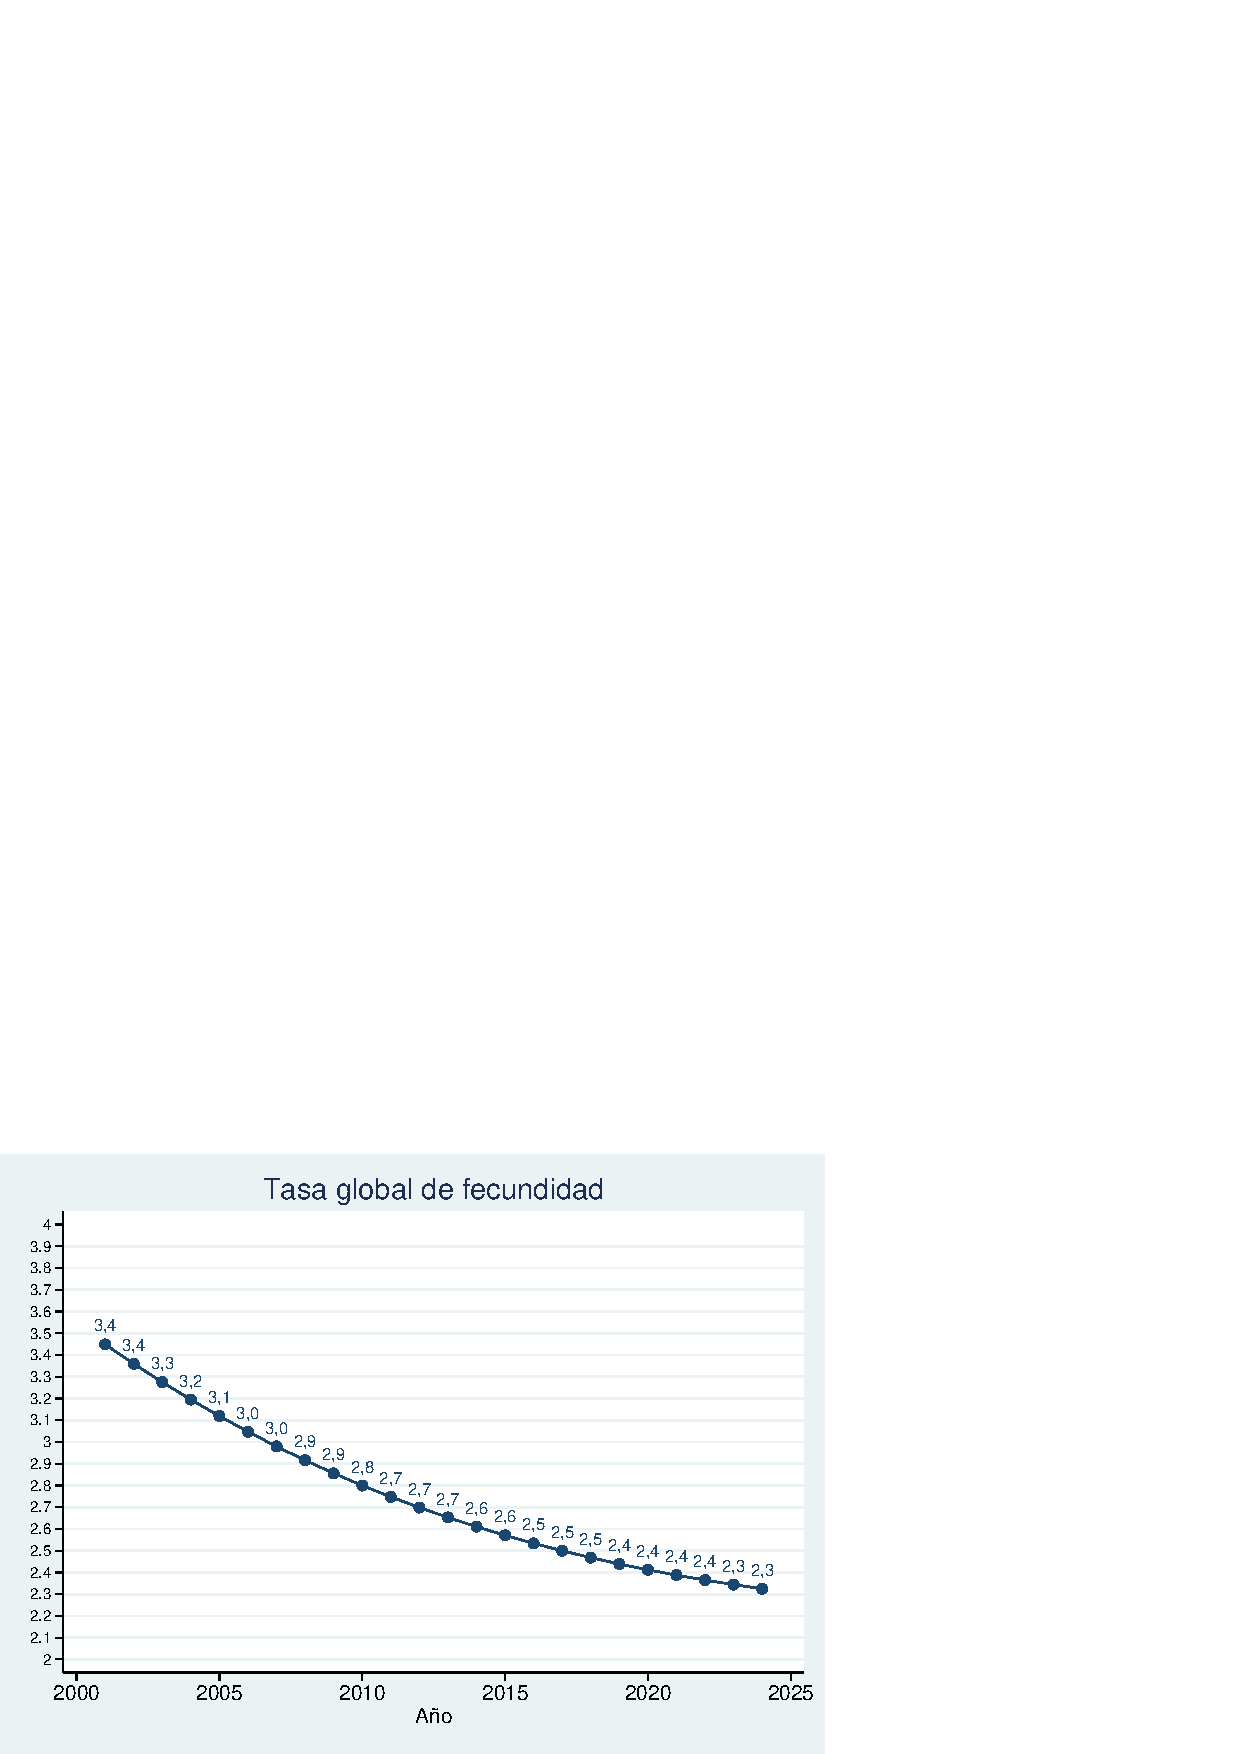
\includegraphics[scale=0.45]{INEtasaglobalfecun.png}
                                    \item \footnotesize Fuente : Instituto Nacional de Estadística.
\end{center}
\end{figure}

\subsubsection{Índice de Masculinidad. Periodo 2000-2025}

El índice de masculinidad, también llamado ``razón de sexo'' es un
índice demográfico que expresa la razón de hombres frente a mujeres en
un determinado territorio, enunciada en tanto por ciento. Se calcula
dividiendo la cantidad total de hombres por la cantidad total de
mujeres.

En el año 2000 había 102,3 hombres por cada 100 mujeres en el Paraguay
\footnote{STP/DGEEC. Paraguay. Proyección de la Población Nacional, Áreas Urbana y Rural por Sexo y Edad, 2000-2025. Revisión 2015.},
estimándose a 101,1 hombres por cada 100 mujeres para el año 2025.

\begin{figure}[H]
\begin{center}
                    \caption{Índice de Masculinidad}
                    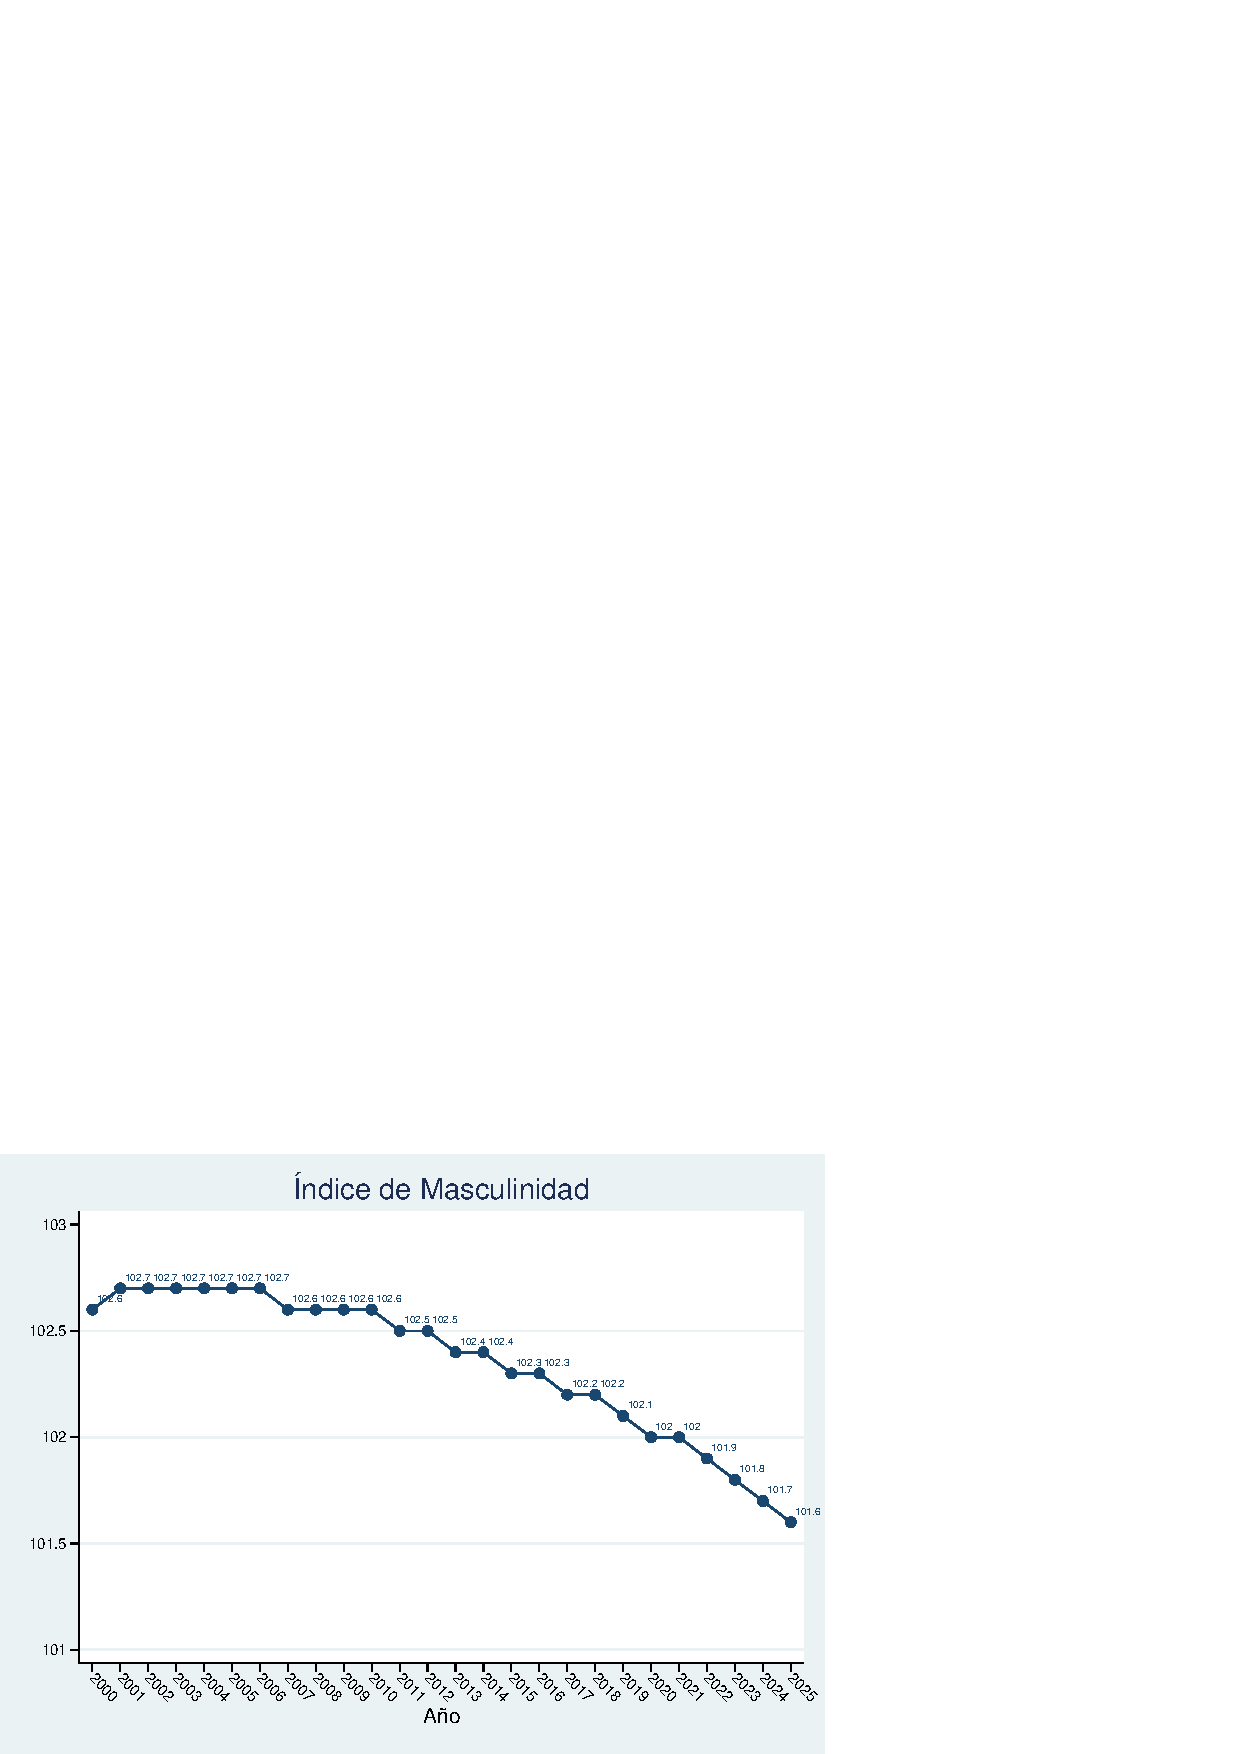
\includegraphics[scale=0.45]{INE_indic_masc.png}
                                    \item \footnotesize Fuente : Instituto Nacional de Estadística.
                    \end{center}
\end{figure}

Esta tasa también es calculada al momento del nacimiento, denominada
Tasa Específica de Masculinidad y es obtenida dividiendo la cantidad de
recién nacidos del sexo masculino con la cantidad de recién nacidos del
sexo femenino.

Al visualizar las tasas global y específica de masculinidad, el interés
recae en la segunda por ser la utilizada como insumo de las proyecciones
actuariales. De los datos históricos y proyectados, se aprecia que la
Tasa Específica de Masculinidad se man tuvo constante en todo el
periodo, promediando un valor muy próximo a 104 hombres por cada 100
mujeres. **** esta evolución no está en el overleaf***

\subsubsection{Migraciones}

El INE ha calculado el saldo neto migratorio recurriendo a varias
fuentes, entre las que se pueden citar los registros oficiales de
entradas y salidas, los censos de población y viviendas nacionales y de
otros países. Como en toda proyección, el saldo m igratorio o migración
neta, es el componente que en principio más influiría en la
incertidumbre respecto al tamaño y estructura futura de la población.

Sin embargo, a menos que se trate de movimientos sustanciales y
persistentes en el tiempo, su efecto no es significativo.

Al observar los datos históricos y la estimación de la migración
internacional neta para el periodo 2001-2025, el Paraguay ha tenido un
saldo negativo en las migraciones netas que fue aumentando hasta el año
2009 donde se observa un cambio en la tendenc ia. A partir del año 2010
ese saldo negativo ha ido disminuyendo y se estima un valor cercano a 0
(cero) para el año 2025.

\begin{figure}[H]
\begin{center}
                    \caption{Migración anual (en miles). Periodo 2001-2025}
                    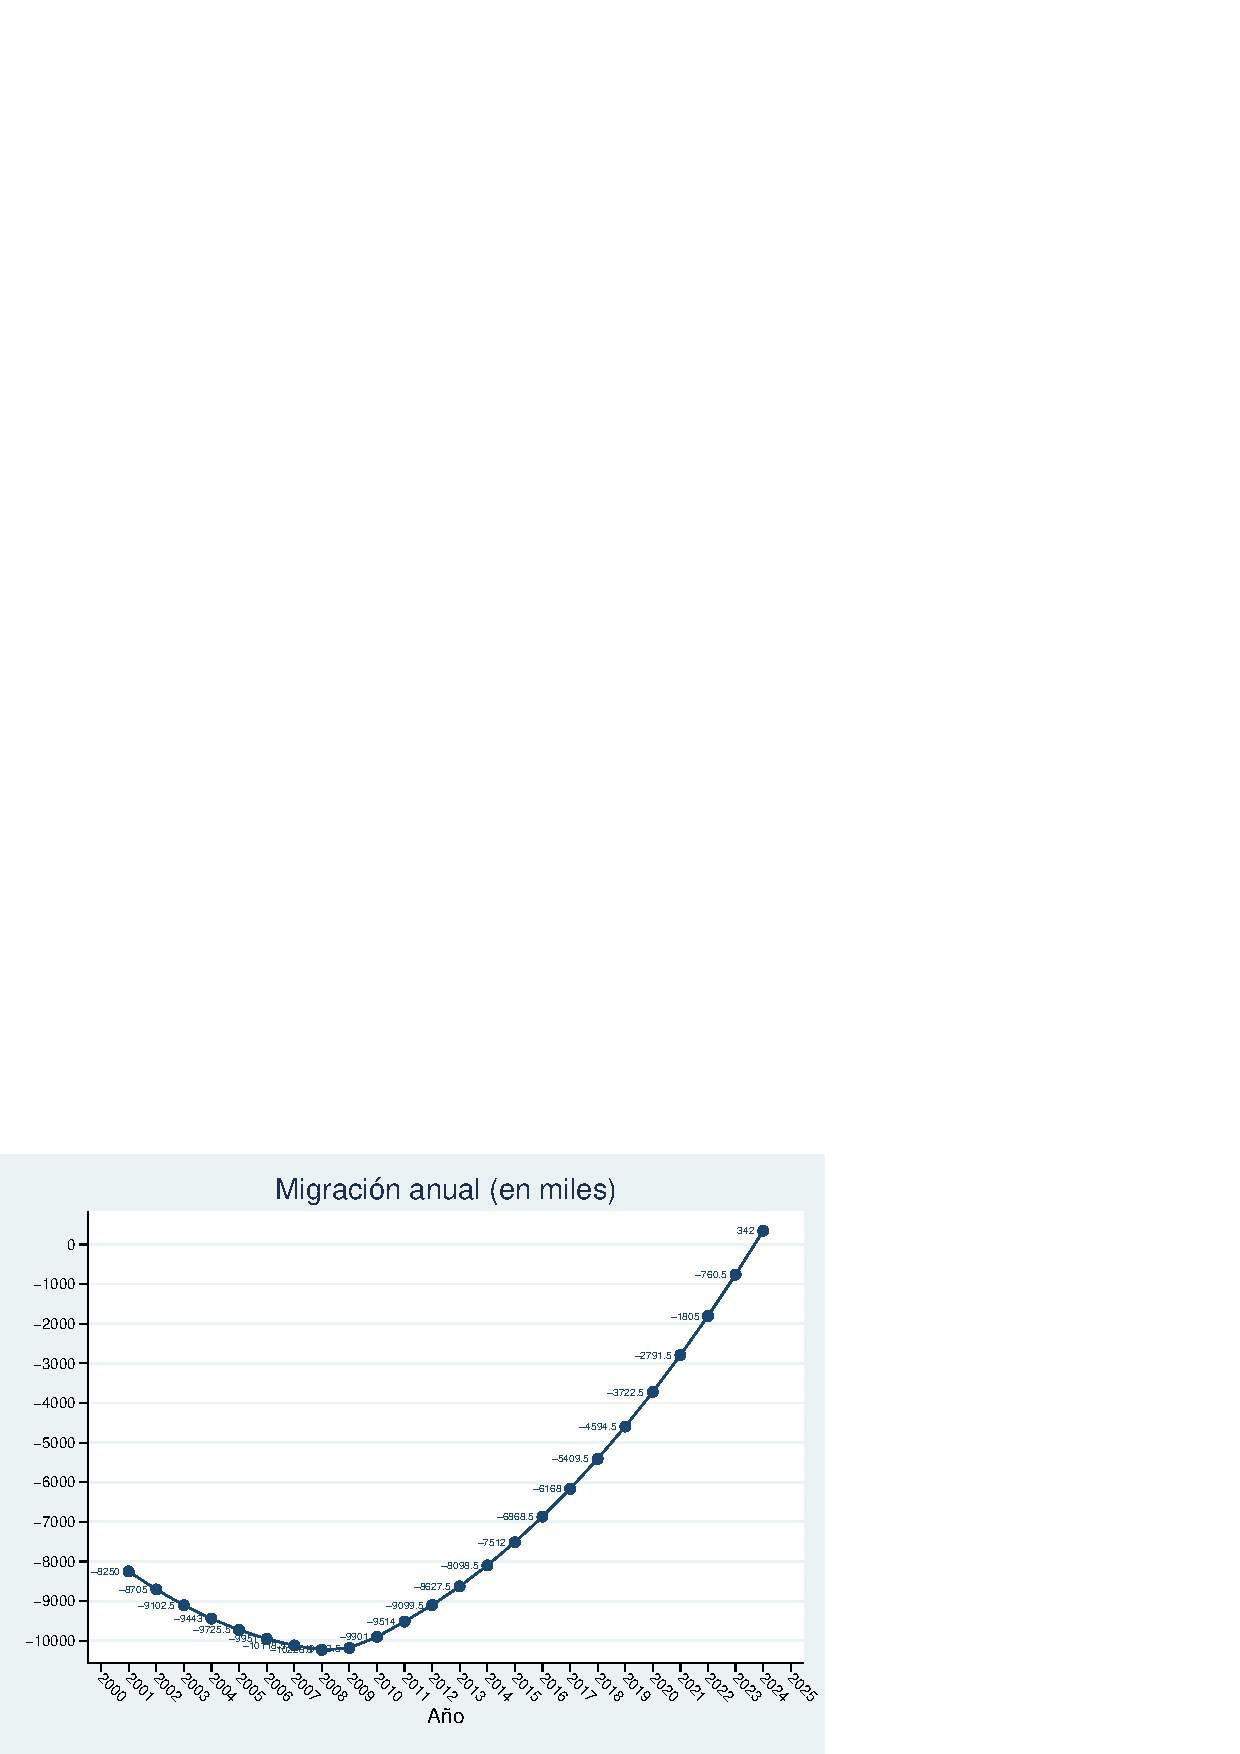
\includegraphics[scale=0.45]{INE_indic_miganaul.png}
                                    \item \footnotesize Fuente : Instituto Nacional de Estadística.
                    \end{center}
\end{figure}

\begin{figure}[H]
\begin{center}
                    \caption{Tasa de migración (por mil). Periodo 2001-2025}
                    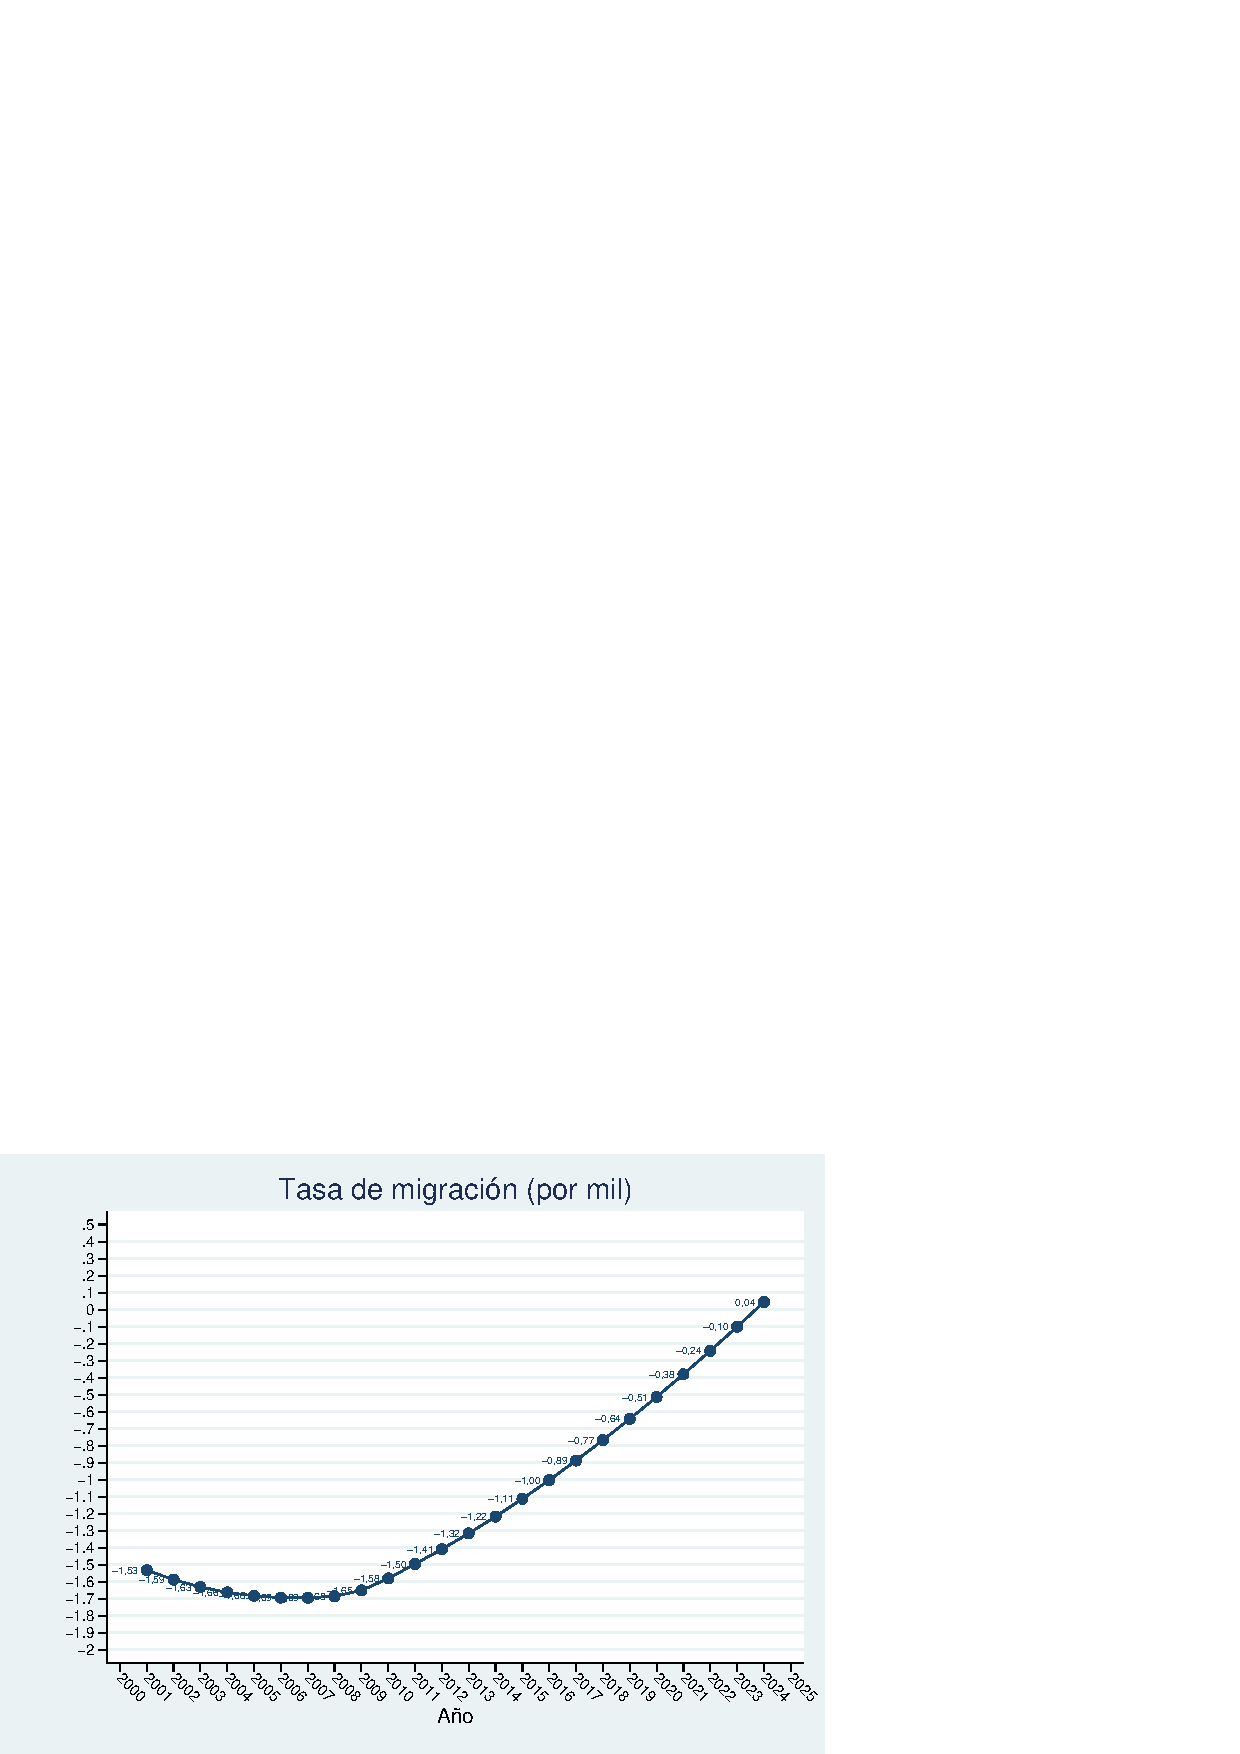
\includegraphics[scale=0.45]{INE_indic_tasamig.png}
                                    \item \footnotesize Fuente : Instituto Nacional de Estadística.
                    \end{center}
\end{figure}
